\section{Propiedades}



\subsection{El estado de máxima entropía general: dos expresiones}
Sea $\rho\in\mcS(\hilbert_{2})$ caracterizado por tres parámetros: su pureza y dos ángulos, $\alpha$ y $\beta$. Su vector de Bloch se puede escribir entonces como
\begin{equation}
  \vec{r}_{\rho}=\text{Pu}(\rho)\begin{pmatrix}
    \cos{\beta}\sin{\alpha}\\
    \sin{\beta}\sin{\alpha}\\
    \cos{\alpha}\\
  \end{pmatrix}=\text{Pu}(\rho)\hat{r}_{\rho}.
\end{equation}
Ahora, sea $\rho_{z}\in\mcS(\hilbert_{2})$ un estado solo con componente en $\sigma_{z}$. La unitaria $V$ tal que $V\rho_{z} V^{\dag}$ tiene la forma
\begin{equation}
  V=
  \begin{pmatrix}
      \cos{\frac{\alpha}{2}} & e^{i\beta}\sin{\frac{\alpha}{2}}\\
      -e^{-i\beta}\sin{\frac{\alpha}{2}}& \cos{\frac{\alpha}{2}},
  \end{pmatrix},
\end{equation}
que en términos de la base de Pauli se ve como
\begin{equation}
  V=e^{i\alpha \hat{l}\cdot \vec{\sigma}}=\Id \cos{\frac{\alpha}{2}}+i(\hat{l}\cdot \vec{\sigma})\sin{\frac{\alpha}{2}},
\end{equation}
con $\hat{l}=(\sin{\beta},\cos{\beta},0)$, y satisface
\begin{equation}\label{eq:VsigmazV}
  V\sigma_{z}V^{\dag}=\sigma_{x}\cos{\beta}\sin{\alpha}+\sigma_{y}\sin{\beta}\sin{\alpha}+\sigma_{z}\cos{\alpha}=\hat{r}_{\rho}\cdot\vec{\sigma}.
\end{equation}
Construyendo $\mcV=V\otimes V$, podemos expresar al estado de máxima entropía de dos formas equivalentes,
\begin{align}\label{eq:MaxEntTwoExpr}
  \boxed{\varrho_{max}(\rho)=\frac{1}{Z}\text{exp}(-\lambda_{3}\mcV\hat{G}_{3}\mcV^{\dag})} && \boxed{\varrho_{max}(\rho)=\frac{1}{Z}\text{exp}(\sum_{i}\lambda_{i}\hat{G}_{i})}
\end{align}

\subsection{El estado máxima entropía es separable}

Sea $\rho_{z}$ un estado alineado en $z$ como en (\ref{eq:rhoz}), entonces por (\ref{eq:MaxEnt}) el estado de máxima entropía es:
\begin{equation}\label{eq:MaxEntUgly}
\varrho_{max}^{z}=\frac{1}{Z}\text{exp}(-\lambda_{3}\hat{G}_{3}),
\end{equation}
donde $\hat{G}_{3}$ se define según (\ref{eq:Gop}). Como los dos términos que componen al operador comuntan entre sí, la exponencial puede separarse como
\begin{align*}
\varrho_{max}^{z}&=\frac{1}{Z}e^{-\lambda_{3}p\sigma_{z}\otimes\Id}e^{-\lambda_{3}(1-p)\Id\otimes\sigma_{z}}\\
&=\frac{1}{Z}(e^{-\lambda_{3}p\sigma_{z}}\otimes\Id)( \Id\otimes e^{-\lambda_{3}(1-p)\sigma_{z}})\\
&=\frac{1}{Z}(e^{-\lambda_{3}p\sigma_{z}}\otimes e^{-\lambda_{3}(1-p)\sigma_{z}}).\\
\end{align*}
Si se separa a la función de partición como un producto de trazas $Z=Z_{1}Z_{2}$, al estado de máxima entropía se le puede escribir como:
\begin{equation}\label{eq:MaxEntZ}
\varrho_{max}^{z}=\frac{e^{-\lambda_{3}p\sigma_{z}}}{Z_{1}} \otimes \frac{e^{-\lambda_{3}(1-p)\sigma_{z}}}{Z_{2}}.
\end{equation}
Esto es válido para el estado alineado en $z$, pero retomando el resultado (\ref{eq:MaxEntTwoExpr}) y la relación (\ref{eq:VsigmazV}), el estado de máxima entropía compatible con un estado grueso arbitrario es
\begin{equation}\label{eq:MaxEntSeparable}
  \boxed{\varrho_{max}=\frac{e^{-\lambda_{3}p(\hat{r}_{\rho}\cdot\vec{\sigma})}}{Z_{1}} \otimes \frac{e^{-\lambda_{3}(1-p)(\hat{r}_{\rho}\cdot\vec{\sigma})}}{Z_{2}}}
\end{equation}
Por lo que el estado de máxima entropía compatible con un estado $\rho$ arbitrario es separable.

\subsection{El estado de máxima entropía bajo la aplicación de grano grueso}\label{sec:CG(MaxEnt)}

El problema de la ecuación (\ref{eq:MaxEntZ}) es que el estado de máxima entropía está en términos del multiplicador de Lagrange que se usó para maximizar la entropía, en lugar de estar en términos de la cantidad medible $\Tr(\rho_{z}\sigma_{z})$. Si por alguna razón tuviéramos que resignarnos a trabajar con el estado en términos de $\lambda_{3}$, será necesario conocer la expresión del estado efectivo. Para hallarla, basta con pasar (\ref{eq:MaxEntZ}) y (\ref{eq:MaxEntSeparable}) por la aplicación de grano grueso. Si el estado grueso está alineado en $z$, entonces tiene la forma
\begin{equation}\label{eq:CG(MaxEntZ)1}
    \rho_{z}=\frac{1}{Z}\CG{\varrho_{max}^{z}}=p\frac{e^{-\lambda_{3}p\sigma_{z}}}{Z_{1}}+(1-p)\frac{e^{-\lambda_{3}(1-p)\sigma_{z}}}{Z_{2}}.
\end{equation}
Las exponenciales de la ecuación (\ref{eq:CG(MaxEntZ)1}) pueden verse como $e^{a\hat{n}\cdot \vec{\sigma}}$. Si se desarollan las series se halla
\begin{equation}\label{eq:PauliVectorExp}
    e^{a\hat{n}\cdot \vec{\sigma}}=\Id \cosh{a}+(\hat{n}\cdot \vec{\sigma})\sinh{a}.
\end{equation}
Así que, sustituyendo la ecuación (\ref{eq:PauliVectorExp}) en (\ref{eq:CG(MaxEntZ)1}) se encuentra la expresión del estado efectivo en términos de la base de Pauli
\begin{align*}
    \rho_{z}&=p\frac{\Id \cosh{\lambda_{3}p}-\sigma_{z}\sinh{\lambda_{3}p}}{Z_{1}}+(1-p)\frac{\Id \cosh{\lambda_{3}(1-p)}-\sigma_{z}\sinh{\lambda_{3}(1-p)}}{Z_{2}}\\
    &=p\frac{1}{2}(\Id \frac{2\cosh{\lambda_{3}p}}{Z_{1}}-\sigma_{z}\frac{2\sinh{\lambda_{3}p}}{Z_{1}})+(1-p)\frac{1}{2}(\Id \frac{2\cosh{\lambda_{3}(1-p)}}{Z_{2}}-\sigma_{z}\frac{2\sinh{\lambda_{3}(1-p)}}{Z_{2}}).
\end{align*}
Para que esto sea de la forma $\rho=\sum_{i}p_{i}\rho_{i}$ es necesario que $Z_{1}=2\cosh{\lambda p}$ y $Z_{2}=2\cosh{\lambda (1-p)}$ (cosa que se puede comprobar). El estado efectivo en términos de $\lambda_{3}$ es
\begin{equation}\label{eq:CG(MaxEntZ)2}
    \rho_{z}=p\frac{1}{2}(\Id+\sigma_{z}\tanh{(-\lambda p)})+(1-p)\frac{1}{2}(\Id+\sigma_{z}\tanh{(-\lambda (1-p))}).
\end{equation}
Naturalmente, el caso general es la ecuación anterior como $V$ aplicada en ella para obtener el estado rotado. Explicitamente
\begin{equation}\label{eq:CG(MaxEnt)}
  \boxed{\rho=\frac{1}{2}[\Id+(\hat{r}_{\rho}\cdot\vec{\sigma})(p\tanh{-\lambda p}+(1-p)\tanh{-\lambda (1-p)})]}
\end{equation}
\notaAd{Esto lo metí en una nota porque no sé qué tan útil fue:

Ahora, si se compara este resultado con la definición de la aplicación de grano grueso y el hecho que el estado de máxima entropía es separable, encontramos que
\begin{align*}
  \varrho_{max}&=\frac{1}{2}(\Id+\sigma_{z}\tanh{(-\lambda p)})\otimes\frac{1}{2}(\Id+\sigma_{z}\tanh{(-\lambda (1-p))})\\
  &  =\frac{1}{4}(\Id_{4}+\sigma_{z}\otimes\Id_{2}\tanh{(-\lambda p)}+\sigma_{z}\otimes \Id_{2}\tanh{(-\lambda (1-p))}+\sigma_{z}\otimes \sigma_{z}\tanh{-(\lambda p)}\tanh{(-\lambda (1-p))})
\end{align*}
}
\subsection{El estado de máxima entropía en términos de la pureza}

La ecuación (\ref{eq:CG(MaxEnt)}) permite expresar la puerza $\text{Pu}(\rho)$ en términos del multiplicador de Lagrange $\lambda_{3}$. En el caso en el que el estado solo tiene componente en $\sigma_{z}$, esto es equivalente a encontrar $r_{z}=\text{Pu}(\rho_{z})$ en términos del multiplicador de Lagrange. Si nos limitamos a dicho caso,
\begin{equation}\label{eq:RzTanh}
    \boxed{r_{z}=p\tanh{-\lambda p}+(1-p)\tanh{-\lambda (1-p)}}
\end{equation}
La ecuación anterior, fijada $p$, es una suma de dos funciones inyectivas, y como tal, es inyectiva también. Esto significa que existe la función inversa.

No se ve ninguna forma sencilla de despejar al multiplicador de Lagrange \notaAd{la ecuación (\ref{eq:RzTanh}) y la ecuación (\ref{eq:RZ}) son completamente equivalentes, como debería de ser. La segunda siendo más fea que la primera. }. En realidad, esto solo se puede si la función $r_{z}(\lambda_{3})$ tiene inversa, y esto puede depender del parámetro $p$. Graficar la superficie (Figura \ref{fig:rzsurf}) puede aclarar algo el panorama.
\begin{figure}[h!]
\centering
\begin{subfigure}{0.475\textwidth}
  \centering
  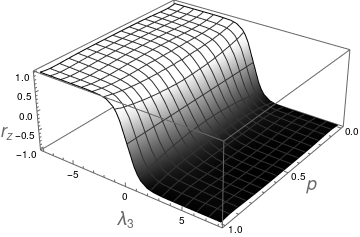
\includegraphics[width=0.6\linewidth]{maxent/figures/LagrangeMult_lambda-8to8.png}
  \caption{$-8<\lambda_{3}<8$}
\end{subfigure}%
\begin{subfigure}{0.475\textwidth}
  \centering
  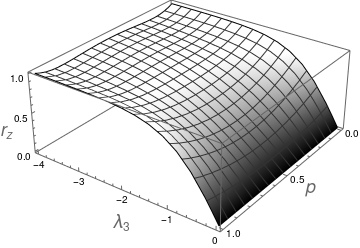
\includegraphics[width=0.6\linewidth]{maxent/figures/LagrangeMult_lambda-4to0.png}
  \caption{$-4<\lambda_{3}<0$}
\end{subfigure}
\caption{Superficie de $r_{z}$ según (\ref{eq:RZ}) para dos intervalos de $\lambda_{3}$. A valores $\lambda_{3}<0$ corresponden valores $r_{z}>0$ y viceversa.}
\label{fig:rzsurf}
\end{figure}

Después de una breve inspección se concluyen las siguientes cosas:
\begin{itemize}
\item la superficie es simétrica respecto al plano $p=0.5$
\item la superficie es antisimétrica  respecto al plano $\lambda_{3}=0$ i.e. $r_{z
}(\lambda_{3},p)=-r_{z
}(-´\lambda_{3},p)$
\item $\text{sgn}(\lambda_{3})=-\text{sgn}(r_{z})$
\end{itemize}

La simetría respecto al plano $p=0.5$ suguiere un cambio de variable $q=\abs{p-0.5}$. La ecuación (\ref{eq:RZ}) se reescribe como:
\begin{equation}\label{eq:RZq}
r_{z}=-\frac{1}{2}\frac{\sinh(\lambda_{3})+2q\sinh(2q\lambda_{3})}{\cosh((q+\frac{1}{2})\lambda_{3})\cosh((q-\frac{1}{2})\lambda_{3})}
\end{equation}
Y nos limitamos al dominio $\lambda_{3}\leq0$ y $0\leq q\leq\frac{1}{2}$. Podemos graficar la función (\ref{eq:RZq}) para diferentes valores de $q$ (Figura \ref{fig:rzinv}).
\begin{figure}[h!]
\centering
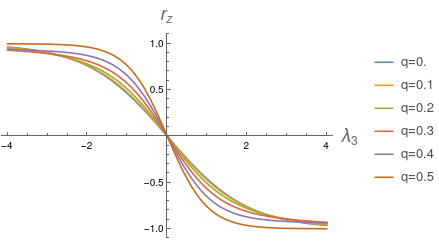
\includegraphics[width=0.6\linewidth]{maxent/figures/rz_has_inverse_lambda-4to4.png}
\caption{$r_{z}$ como función de $\lambda_{3}$ para diferentes valores de $q$. La apariencia uno a uno sugiere la existencia de una inversa.}
\label{fig:rzinv}
\end{figure}

\subsubsection{Dos soluciones particulares}

Considerando el caso $q=\frac{1}{2}$, la ecuación (\ref{eq:RZq}) se reduce a 
\begin{equation}
r_z=-\frac{1}{2}\frac{2\sinh(\lambda_{3})}{\cosh(\lambda_{3})}
\end{equation}
de manera que $\lambda_{3}=-\text{arctanh}(rz)$.

Si $q=0$, la ecuación (\ref{eq:RZq}) se reduce a
\begin{equation}
r_z=-\frac{\sinh(\lambda_{3})}{\cosh(\lambda_{3}+1)}
\end{equation}
Mathematica sugiere la solución:
\begin{equation}\label{eq:lambda0.5}
\lambda_{3}=\log\qty(\frac{1-r_{z}}{1+r_{z}}).
\end{equation}
\newpage